\section{HTTP Method Request}
\subsection{Pengertian HTTP Method Request}
Protokol HTTP adalah protokol permintaan atau respon. Klien mengirimkan permintaan keserver dalam bentuk metode permintaan, URL, dan versi protokol, diikuti oleh pesan seperti MIME yang berisi perubahan permintaa, informasi klien, dan kemungkinan onten tubuh melalui koneksi dengan server\cite{wyler2005aggressive}. Protokol ini sangat ringan serta generik dan tidak berstatus sehingga dapat dipergunakan oleh tipe dokumen apa saja. Method adalah sekumpulan kode yang diberi namma, untuk merujuk kesekumpulan kode yang ada kemuadian digunakan sebuah nama yang disebut dengan nama method. Method sendiri mempunyai parameter sebagai input (masukan) dan nilai kembalian sebagai output (keluaran). Request adalah permiintaan dimana fungsi ini digunakan sebagai istilah ataupun kinerja dalam pengembalian nilai dari masukan yang dieksekusi.

Berdasarkan beberapa penjelasann diatas, maka untuk pengertian dari HTTP Method Request sendiri merupakan seperangkat metode permintan untuk menunjukkan tindakan yang diinginkan yang akan dilakukan untuk sumber daya tertentu. Meskipun mereka juga bisa menjadi kata benda, metode permintaan ini kadang-kadang disebut sebagai verba HTTP. Masing-masing menerapkan semantik yang berbeda, namun beberapa fitur umum digunakan bersama oleh mereka adalah misalnya Metode pertmintaan dapat berupa safe, idempotent, atau cacheable.

\subsection{Jenis-jenis HTTP Method Request}
\begin{enumerate}
  \item GET : akan dijelaskan pada point berikutnya.
  \item HEAD : Metode HEAD meminta tanggapan yang identik dengan permintaan GET, namun tanpa respon body.
  \item POST : Metode POST digunakan untuk mengirimkan entitas ke sumber daya yang ditentukan, sering menyebabkan perubahan pada keadaan atau efek samping pada server.
  \item PUT : Metode PUT menggantikan semua representasi terkini dari sumber target dengan muatan permintaan.
  \item DELETE : Metode DELETE akan menghapus sumber daya yang ditentukan
  \item CONNECT : Metode CONNECT menetapkan terowongan keserver yang diidentifikasi oleh sumber target.
  \item OPTIONS : Metode OPTIONS digunakan untuk menggambarkan opsi komunikasi untuk sumber target.
  \item TRACE : metode TRACE ini yaitu untuk melakukan tes pesan loop-back disepanjang jalan menuju sumber daya target.
  \item PATCH : Metode PATCH digunakan untuk menerapkan modifikasi sebagian pada sumber daya.
\end{enumerate}

\subsection{Penjelasan Lengkap HTTP Get Method}
Metode GET digunakan untuk meminta representasi suber daya yang ditentukan. permintaan menggunakan Get seharusnya hanya mengambil data. GET adalah salah satu metode HTTP yang paling umum digunakan baik dalam pengimplementasian biasa ataupun sudah dalam bentuk pengujian. Hal yang harus diperhatikan dalam Method Get yaitu :
\begin{itemize}
  \item Permintaan GET dapat di-cache.
  \item Permintaan GET tetap ada dalam riwayat browser.
  \item Permintaan GET dapat ditandai.
  \item Permintaan GET tidak boleh digunakan saat berurusan dengan data sensitif.
  \item Permintaan GET memiliki batasan panjang.
  \item Permintaan GET hanya digunakan untuk meminta data (tidak dimodifikasi).
  \item Permintaan GET dibatasi oleh panjang string sebanyak 2047 karakter.
  \item Permintaan GET memungkinkan pengunjung langsung memasukkan nilai variable pada form proses.
\end{itemize}

\subsection{Pembacaan HTTP Get Method}
Data dikirimkan dalam HTTP Request dalam dua cara, tergantung dari method yang dikirimkan, yaitu :
\begin{enumerate}
  \item Melalui URL, dengan parameter yang diberikan. Digunakan oleh GET.
  \item Melalui entity body dalam HTTP Request. Digunakan untuk POST dan PUT.
\end{enumerate}

Pada prakteknya terdapat satu cara lagi untuk mengirimkan data, yaitu melalui cookie, tetapi penggunaan cookie tidak akan terlalu efektif karena cookie dirancang untuk menyimpan data status pengguna.

\subsection{Pembacaan Data pada URL}
Pembacaan data yang dikirimkan melalui URL biasanya dilakukan untuk request dengan method GET. Untuk melihat bagaimana GET mengirimkan data, kita terlebih dahulu harus mengerti tentang sintaks penulisan URL. Secara umum, sebuah URL memiliki sintaks seperti berikut :
\lstinputlisting[caption=Contoh kode untuk schema,label={lst:schema}]{src/10/schema.py}
Apa makna dari setiap bagian dari URL yang dijelaskan pada \ref{lst:schema}? Pada tabel \ref{table:schema}, anda dapat melihat makna dan maksud dari contoh URL yang telah diberikan.
\begin{table}[]
\caption{Penjelasan Schema}
\centering
\begin{tabular}{|l|l|l|}
\hline
Nama & Deskripsi & Harus ada ?\\ \hline
schema & Protokol yang digunakan & Ya\\ \hline
user & Nama pengguna & Tidak\\ \hline
password & Password untuk nama pengguna & Tidak\\ \hline
hots & Hostname atau IP & Ya\\ \hline
port & \begin{tabular}[c]{@{}l@{}}Port yang akan diakses. Beberapa atau sebagian\\ protokol memiliki port standar yaitu seperti HTTP = 80\end{tabular} & Tergantung Protokol\\ \hline
paht & Lokasi data pada server & Tergantung Protokol\\ \hline
query & \begin{tabular}[c]{@{}l@{}}Digunakan untuk mengirimkan \\ parameter kepada aplikasi.\end{tabular} & Tidak\\ \hline
fragment & \begin{tabular}[c]{@{}l@{}}Nama dari bagian tertentu pada \\ data (misalnya : judul pada buku)\end{tabular} & Tidak\\ \hline
\end{tabular}
\label{table:schema}
\end{table}

\section {Mekanisme HTTP Method Request}
\subsection{Mekanisme / Alur kerja HTTP Get Method}
Mekanisme adalah suatu rangkaian kerja sebuah alat yang digunakan dalam menyelesaikan sebuah masalah yang berkaitan dengan proses kerja, tujuannya untuk menghasilkan hasil yang mekasimal serta mengurangi datangnya atau munculnya kegagalan. untuk mekanisme HTTP Get Method sendiri dapat diperhatikan sebagai berikut :
\begin{enumerate}
  \item Silahkan membuat dan membangun sebuah URL API.
  \item Didalam URL API (endpoint) tersebut kita akan menggunakan fungsi Method Get.
  \item Kemudian didalam endpoint tersebut akan difungsikan inputan.
  \item Inputan tersebut kemudian akan meghasilkan output (keluaran) dari Metgod GET tersebut.
  \item Secara sederhana, garis besar mekanisme atau alur kerja Method Get nampak seperti penjelasan diatas.
  \item Untuk tutorial pembangunan endpoint seperrti pada point kedua akan dijelaskan pada point selanjutnya.
\end{enumerate}

\section {Contoh URL HTTP Get Method}
Untuk pemberian contoh ini akan dibarengin dengan tutorial pembangunannya, jadi diharapkan teman-teman dapat dengan mudah memahami dan mudah dalam mengikuti contoh yang diberikan. Berikut tutorialnya :
\begin{enumerate}
  \item Endpoint adalah perangkat komputasi jarak jauh yang berkomunikasi bolak-balik dengan jaringan yang terhubung dengannya. Fungsi-fungsi yang dipergunakan yaitu sebagai contoh berikut :
      \begin{itemize}
        \item Fungsi 1 : LoadData.py yaitu membaca file CSV.
            \lstinputlisting[caption=Contoh kode untuk membaca file CSV,label={lst:LoadData}]{src/10/LoadData.py}
        \item Fungsi 2 : Getalldata.py yaitu untuk menampilkan semua data dari file CSV.
            \lstinputlisting[caption=Contoh kode untuk menampilkan semua data dari file CSV,label={lst:GetAllData}]{src/10/GetAllData.py}
        \item Fungsi 3 : Getcolumn.py yaitu untuk menampilkan data dari kolom tertentu.
            \lstinputlisting[caption=Contoh kode untuk menampilkan data dari kolom,label={lst:Getcolumn}]{src/10/Getcolumn.py}
        \item Fungsi 4 : Gettopfive.py yaitu untuk menampilkan 5 data teratas dan terbawah.
            \lstinputlisting[caption=Contoh kode untuk menampilkan 5 data teratas dan terbawah,label={lst:Gettopfive}]{src/10/Gettopfive.py}
        \item Fungsi 5 : Sorting.py yaitu untuk mengurutkan data dari yang terbesar ke yang terkecil dan sebaliknya.
            \lstinputlisting[caption=Contoh kode untuk mengurutkan data,label={lst:Sorting}]{src/10/Sorting.py}
        \item Fungsi 6 : Convertjson.py yaitu untuk mengganti data kedalam format Json.
            \lstinputlisting[caption=Contoh kode untuk mengganti data,label={lst:Convertjson}]{src/10/Convertjson.py}
        \item Fungsi 7 : Deletecolumn.py yaitu untuk menghapus kolom tertentu.
            \lstinputlisting[caption=Contoh kode untuk menghampus kolom tertentu,label={lst:Deletecolumn}]{src/10/Deletecolumn.py}
        \item Fungsi 8 : Deletealldata.py yaitu untuk Menghapus semua data pada file CSV.
            \lstinputlisting[caption=Contoh kode untuk menghapus semua data,label={lst:Deletealldata}]{src/10/Deletealldata.py}
        \item Fungsi 9 : Insertdata.py yaitu untuk menambahkan data.
            \lstinputlisting[caption=Contoh kode untuk menambah data,label={lst:Insertdata}]{src/10/Insertdata.py}
        \item Fungsi 10 : Getinfo.py yaitu untuk Menampilkan data csv namun dengan format json bawaan dari library pandas yang akan berupa deskripsi.
            \lstinputlisting[caption=Contoh kode untuk Menampilkan data csv,label={lst:Getinfo}]{src/10/Getinfo.py}
        \item Fungsi 11 : Getrow.py yaitu untuk Menampilkan seluruh jumlah baris.
            \lstinputlisting[caption=Contoh kode untuk Menampilkan seluruh jumlah baris,label={lst:Getrow}]{src/10/Getrow.py}
        \item Fungsi 12 : Getrowfield.py yaitu untuk Menampilkan data perbaris sesuai dengan kolom yang diiginkan.
            \lstinputlisting[caption=Contoh kode untuk Menampilkan data perbaris,label={lst:Getrowfield}]{src/10/Getrowfield.py}
        \item Fungsi 13 : Updatedata.py yaitu untuk Mengubah data berdasarkan index id.
            \lstinputlisting[caption=Contoh kode untuk Mengubah data berdasarkan index id,label={lst:Updatedata}]{src/10/Updatedata.py}
        \item Fungsi 14 : Deletedata.py yaitu untuk Menghapus data berdasarkan index id.
            \lstinputlisting[caption=Contoh kode untuk Menghapus data berdasarkan index id,label={lst:Deletedata}]{src/10/Deletedata.py}
        \item Fungsi 15 : Getrowjson.py yaitu untuk Mengubah data menjadi Json.
            \lstinputlisting[caption=Contoh kode untuk Mengubah data menjadi Json,label={lst:Getrowjson}]{src/10/Getrowjson.py}
        \item Fungsi 16 : Getalldatajson.py yaitu untuk Menampilkan seluruh data dalam bentuk format Json.
            \lstinputlisting[caption=Contoh kode untuk Menampilkan seluruh data,label={lst:Getalldatajson}]{src/10/Getalldatajson.py}
        \item Fungsi 17 : Amountdata.py yaitu untuk Menghitung jumlah data secara keseluruhan dari kolom dan baris.
            \lstinputlisting[caption=Contoh kode untuk Menghitung jumlah data,label={lst:Amountdata}]{src/10/Amountdata.py}
        \item Fungsi 18 : Getcolumncount.py yaitu untuk Menghitung jumlah kolom pada file.
            \lstinputlisting[caption=Contoh kode untuk Menghitung jumlah kolom,label={lst:Getcolumncount}]{src/10/Getcolumncount.py}
        \item Fungsi 19 : Getrowcount.py yaitu untuk Menghitung jumlah baris pada file.
            \lstinputlisting[caption=Contoh kode untuk Menghitung jumlah baris,label={lst:Getrowcount}]{src/10/Getrowcount.py}
        \item Fungsi 20 : Reloaddata.py yaitu untuk Mengembalikan nilai data.
            \lstinputlisting[caption=Contoh kode untuk Mengembalikan nilai data,label={lst:Reloaddata}]{src/10/Reloaddata.py}
      \end{itemize}

  \item Endpoint 1 (URL API / Dataset)
  Pembatasan pertama ialah dari Endpoint 1 dimana URL API nya yaitu dataset. Silahkan tuliskan code dibawah sebagai contoh pertama :
  \lstinputlisting[caption=Contoh kode untuk URL API,label={lst:MethodGetfromEndpoint}]{src/10/MethodGetfromEndpoint.py}

  Pada tabel code diatas dapat dilihat bahwa fungsi yang digunakn ialah dataset dimana data set dilakukan pemaggilan fungsi yang ada di file-file yang telah di import. Seperti yang bisa dilihat bahwa pada fungsi dataset direalisasikan dengan metode GET, POST dan DELETE jadi disesuaikan dengan fungsi pada file-file yang dihubungkan atau dipanggil kedalam fungsi dataset. Yang akan dibahas disini adalah MEthod GETnya saja. Tutorialnya sebagai berikut :
  \begin{itemize}
    \item Setelah melakukan perintah \ref{lst:MethodGetfromEndpoint}
    \item Kemudian masukkan perintah yang sesuai
    \item Pendefinisian endpoint dataset
    \item Definisikan request atau permintaan metode yang digunakan. Ada Get 
    \item Pada Method GET : Silahkan masukkan beberapa argument yang akan diolah.
    \item Argumentnya ialah parameter field, topfive, sort dan format
    \item Penjelasan Parameter :
        \subitem All : Mengambil semua data dari file csv
        \subitem Field : Mengambil data berdasarkan parameter field yaitu ada RawValue, sign dan daya
        \subitem Topfive : Mengambil 5 data berdasarkan data paling atas dan 5 data paling bawah
        \subitem Sort : Mengambil data dan diurutkan sesuai dengan urutan ascending (kecil ke besar) dan descending (besar ke kecil)
        \subitem Format : Menampilkan data dengan format tulisan JSON dan Raw
    \item Selanjutnya pastikan setiap argument memberikan respon sesuai dengan fungsi masing-masing 
    \item Kemudian reloaddata akan menampilkan data terbaru setelah dilakukan perintah delete
    \item Silahkan uji endpointnya sesuai dengan parameter tersebut menggunakan POSTMAN maka hasilnya akan seperti berikut :
        
  \end{itemize}
\end{enumerate}

\section {Mendapatkan Parameter GET Python Flask}
    \begin{enumerate}
        \item Pengenalan Python
        Python adalah salah satu bahasa pemograman tingkat tinggi yang bersifat interpreter, interactive, objectoriented, dan dapat beroperasi hampir di semua platform: Mac, Linux, dan Windows. Python termasuk bahasa pemograman yang mudah dipelajari karena sintaks yang jelas, dapat dikombinasikan dengan penggunaan modulmodul siap pakai, dan struktur data tingkat tinggi yang efisien \cite{kadir2005dasar}. Python mendukung multi paradigma pemrograman, utamanya; namu tidak dibatasi; pada pemrograman berorientasi objek, pemrograman imperatif, dan pemrograman fungsional. Salah satu fitur yang tersedia pada python adalah sebagai bahasa pemrograman dinamis yang dilengkapi dengan manajemen memori otomatis.

        Seperti halnya pada bahasa pemrogrman dinamis lainnya, python umumnya digunakan sebagai bahasa skrip meski pada praktiknya penggunaan bahasa ini lebih luas mencakup konteks pemanfaatan yang umumnya tidak dilakukan dengan menggunakan bahasa skrip. Python dapat digunakan untuk berbagai keperluan pengembangan perangkat lunak dan dapat berjalan di berbagai platform sistem operasi.

        \item Pengenalan Flask
         Flask adalah \textit{Web Application Framework} yang ditulis dalam bahasa pemrograman Python. Flask digunakan untuk mempersingkat dan mempermudah pengembangan \textit{Web Application}\cite{lokhande2015efficient}. Flask disebut micro framework karena tidak membutuhkan alat-alat tertentu atau pustaka. Flask tidak memiliki database abstraction layer, validasi form, atau komponen lain dimana sudah ada database pihak ketiga yang menyediakan fungsi umum.

        \item Penjelasan Parameter GET Python Flask
        Parameter GET pada Python Flask ini dilampurkan dan diujikan dalam bentuk file penuh dengan beberapa fungsi. File tersebut bernama Main.py. Untuk penerapan lebih dan contoh GETnya sudah ditampilkan dan dijelaskan sebelumnya pada point contoh URL GET. Namun, penggabungannya bersama Flask Python ada pada file ini. Perhatikan penjelasan dan tutorialnya agar dapat dimengerti. Namun sebelum melanjutkan tutorialnya, pertama-tama anda harus memastikan beberapa hal yaitu sebagai berikut :
    \end{enumerate}

\section{Macam-Macam Penanganan Error Proyek}
\subsection{Penanganan Error pada Python dan Flask}
\begin{enumerate}
  \item Contoh Kasus 1 : Penerapan fungsi sederhana yang dieksekusi dicommand prompt. Contoh pemanggilan fungsi apabila dieksekusi di CMD, seperti gambar \ref{fig:contohsederhana}

  \begin{figure}[!ht]
        \centerline{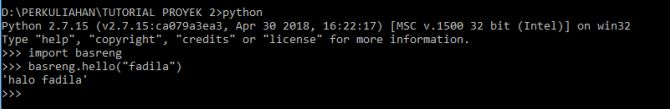
\includegraphics[width=0.85\textwidth]{figures/10/contohsederhana.jpg}}
	    \caption{Fungsi Sederhana}
	    \label{fig:contohsederhana}
  \end{figure}

ini adalah contoh untuk pengeksekusian file python yang berupa gunsi yang telah dibuat. Berikut langkah-langkahnya :
    \begin{itemize}
        \item Petama-tama masukkan kedalam directory tempat anda menyimpan file yang telah anda buat.
        \item kemudian pada directory tersebut ketik python
        \item Setelah masuk kedalam python silahkan masukkan file python basreng
    \end{itemize}

  \item Contoh kasus 2 : Kode pembawa sinyal gelombang otak (NeuroSky Mindwave EEG). Kodenya seperti contoh \ref{lst:coba}, silahkan tutorialnya diikuti terlebih dahulu.
\lstinputlisting[caption=Contoh kode untuk membaca sinyal gelombang otak,label={lst:coba}]{src/10/coba.py}
\end{enumerate}
\begin{itemize}
\item Script Code pada listing \ref{lst:coba} mendefinisikan perintah dimana fungsinya akan dipanggil dan berhubungan dengan mindwave.py
\item Seperti contoh perintah headset.connect dimana fungsinya akan diproses di mindwave.py sehingga apabila hasilnya benar dan sesuai maka akan muncul kata “connecting” seperti perintah print diatas
\item Apabila alat dan code sesuai maka fungsinya akan jalan, baik itu connected, standby dll.
\item Untuk pembacaan sinyalnya, kita menggunakan variabel dari mindwave.py 
\item Untuk variabelnya bisa dicoba yang attention / blink / meditation dll secara bersamaan juga bisa asal perintahnya benar. 
\item Perhatikan script code pada listing \ref{lst:coba1} ini :
\lstinputlisting[firstline=5, lastline=6, caption=Contoh1 kasus 2,label={lst:coba1}]{src/10/coba.py}
\item Untuk mengkoneksikan code dengan alat sehingga terhubung maka serial dari alat tersebut harus benar. Portnya yaitu COM4 dapat dilihat dengan cara :
\begin{enumerate}
\item Buka pengaturan laptop anda 
\item Kemudian pilih device manager 
\item Lalu pilih alat yang anda gunakan misalnya : Mindwave Neurosky 
\item Apabila telah diklik maka akan muncul portnya yaitu COM4  
\item Untuk serialnya dapat dilihat dari alatnya sendiri  
\item Pengecekannya yaitu di dalam tempat baterai. Serialnya 1425 g. Port dan serial itu beda-beda tergantung dari alatnya masing-masing 
\end{enumerate}
\item Time.sleep itu gunanya untuk memberikan jeda pembacaan sinyal sehingga nilai gelombang yang dibaca tidak terlalu cepat dan dapat lebih terpantau. Lebih jelasnya lagi, mengapa time.sleepnya bernilai ( 0.001953125 ) dikarenakan : 
\item Silahkan perhatikan ini :
%Tabel 3. Contoh 2 kasus 2 print "raw_value: %s" % (headset.raw_value)  time.sleep(0.001953125) 
%Gambar 3. Sampling contoh kasus 2 
\item Sampling rate dari alat yang digunakan ialah 512Hz jadi tentunya kita harus mengikuti dan menyesuaikannya dengan baik, untuk code dan alatnya.
\item Kemudian 512Hz tersebut kita bagi dengan 1 ( detik ) jadi hasilnya akan menjadi jeda antara sinyal yang telah ditangkap/ dibaca dari alat.
\item 1/512 = 0.001953125 . Nilai itu yang akan menjadi jeda pada code. 
\item Selain itu. Kita juga harus memastikan apakah benar bahwa dalam 1 detik itu ada 512 data yang dibaca dan ditangkah oleh alat.
\item Dan sesuai hasil dari penguijannya sudah dibuktikan dalam setiap detiknya ada sekitar 480-520an data perdetik 
\end{itemize}
 
Setelah semua langkah di atas telah dilakukan, kita akan mencoba running coba.py melalui cmd, dengan cara :
\begin{itemize}
\item Buka Command Prompt di komputer/laptop anda masing-masing 
\item Silahkan pada CMD arahkan ke folder / directory tempat file coba.py anda simpan 
\item Namun sebelum itu pastikan alat sudah terpasang baterai dan lampu indikator berwarna merah 
\item Masukkan USB ke port yang ada di laptop anda. USBnya tentu milik dari alat mindwavenya 
\item Kemudian silahkan masukkan perintah python coba.py 
\item Apabila pas anda jika terjadi ERROR seperti gambar dibawah ini   
%Gambar 4. Error 1 contoh kasus 2 
 \item ERROR diatas sebenarnya menunjukan bahwa indentasi codingan anda tak sesuai maka yang perlu dilakukan ialah rapikan code anda sesuai dengan perintah-perintah terkait. Biasanya ERROR ini terjadi ketika code anda tak berada pada tempatnya maka silahkan sesuaikan dengan SPACI ataupun TAB. 
\item Silahkan Run kembali
\item Ketika di Run, dan terjadi ERROR ditengah jalan seperti ini lagi : 
%Gambar 5. Error 2 contoh kasus 2 
\item Maka anda harus menerapkan Try and Except pada codingan mindwavenya 
\item Contohnya seperti berikut : 
%Tabel 4. Try and Except if code == RAW_VALUE:   try:    anu = value[0]    itu = value[1]   except IndexError:    anu = "0"    itu = "0" 
\item Penggunaan try dan except yaitu untuk menangani error pada code yang dihindari untuk terjadi ketika sedang membaca sinyal  
\item Dimisalkan penangangan errornya untuk penanganan index 
\item Selain index sebenarnya bisa juga untuk menangani error pada IO, database, dictionary dan lain-lain. 
\item Setelah penerapan tersebut silahkan re-run file coba.py 
\item Maka tidak akan terjadi error lagi 
\end{itemize}

Contoh kasus 3: Code fungsi Python sederhana ( silahkan diikuti tutorialnya terlebih dahulu )

1. ( ERROR 1 ) : Fungsi di definisikan dalam Python dengan def. Setelah def ada nama pengenal fungsi diikut dengan parameter yang diapit oleh tanda kurung dan diakhir dingan tanda titik dua ( : ). Baris berikutnya berupa blok fungsi yang akan dijalankan jika fungsi dipanggil. Perhatikan script code pada listing ]ref{lst:hello1} :
\lstinputlisting[caption=Fungsi hello1.py untuk error 1,label={lst:hello1}]{src/10/hello1.py}

Berdasarkan code diatas, telah didefinisikan fungsi berupa hello dimana parameternya yaitu nama. Kemudian terdapat 2 variabel baru yang dijadikan inputan pada fungsi tersebut. lebih jelasnya dapat membaca dan mengikuti langkah-langkah di bawah ini : 
\begin{itemize}
\item Pertama-tama silahkan buat file python dengan nama basreng.py 
\item Selanjutnya buat fungsi bernama hello 
\item Kemudian buka kurung lalu diisi dengan parameter “nama” kemudian tutup kurung lagi 
\item Jangan lupa untuk memberikan titik dua pada perintah sehingga dapat terbaca dan dijalankan 
\item Silahkan inputkan perintah yang ingin dieksekusi dalam fungsi hello 
\item Dimisalkan pada contoh diatas dibuatkan variabel “sambutan” 
\item Variabel “sambutan” di definisikan dengan keluaran string “halo” 
\item Kemudian buatlah variabel baru dengan nama “gabung” 
\item Setelah itu pada variabel “gabung” masukkan variabel “sambutan” lalu tambahkan tanda (+) lalu masukkan perintah nama
\item Setelah itu masukkan perintah return 
\item Pada perintah return ikutkan variabel yang ingin dieksekusi dan lihatlah keluarannya (output) 
\item Karena yang dikembalikan adalah variabel “gabung” maka hasilnya akan berupa “halo (nama yang anda masukkan)” . misal : Halo Fadila. 
\item Itu adalah hasil yang diiginkan, namun 
\item Ketika telah mengikuti tutorial diatas, dan diuji di cmd, hasilnya seperti ini. 
\item Terjadi ERROR. Kita lihat Error berikut : 
%Gambar 6. Error 1 untuk error 1 pada contoh kasus 3 
\item Errornya bertuliskan : IndentationError: expected an indented block
\item Arti dari ERROR tersebut ialah, identasi dan penempatan dari fungsinya tidak sesuai.  
\end{itemize}

Code python sangatlah sensitif jadi penempatannya harus sesuai. Penanganannya yaitu silahkan terapkan TAB atau SPACI sehingga perintahnya sesuai dan dapat dieksekusi sehingga mengikuti perintah-perintah yang berkaitan lainnya.
\begin{itemize}
\item Code yang benar seperti berikut : 
Tabel 6. Fungsi hello 2 untuk error 1  
\begin{verbatim}
def hello(nama): 
	sambutan = "halo" gabung = sambutan + " " + nama 
 	return gabung 
\end{verbatim}
\item Maka ketika kita menguji ulang pada CMD, hasilnya akan seperti berikut: 
%Gambar 7. Penyelesaian untuk error 1 pada contoh kasus 3 
\item Keluarannya benar, yaitu Halo Fadila 
\end{itemize}